% LTeX: language=fr
\documentclass[12pt,twoside]{report}
\usepackage[language=fr,link, quote, floatbarrier, geometry=1]{main}
\usepackage[titlenum=2,fancytitle=3,fancypage=4, name={Benjamin Stambach \ MIQ3} ]{styles}
\usepackage[actif=false]{adddoc}

\usepackage{lipsum}
\newcommand{\eqtest}{\lipsum[1][1-3]
\begin{align*}
    J = \begin{bmatrix}
        -r_1 \sin(q_1) & r_2 \sin(q_2) & -r_3 \sin(q_3) & r_4 \sin(q_4)  \\
        r_1 \cos(q_1) & -r_2 \cos(q_2) & r_3 \cos(q_3) & -r_4 \cos(q_4)  \\
        -r_1 \sin(q_1) & 0 & -r_6 \sin(\alpha+q_3) & 0 \\
        r_1 \cos(q_1) & 0 & r_6 \cos(\alpha+q_3) & 0  \\
    \end{bmatrix} 
    \end{align*}
\lipsum[1][1-3]}
\newcommand{\eqtestsp}{\lipsum[1][1-3]
\begin{align*}
    J = \begin{bmatrix}
        -r_1 \sin(q_1) & r_2 \sin(q_2) & -r_3 \sin(q_3) & r_4 \sin(q_4)  \\
        r_1 \cos(q_1) & -r_2 \cos(q_2) & r_3 \cos(q_3) & -r_4 \cos(q_4)  \\
        -r_1 \sin(q_1) & 0 & -r_6 \sin(\alpha+q_3) & 0 \\
        r_1 \cos(q_1) & 0 & r_6 \cos(\alpha+q_3) & 0  \\
    \end{bmatrix}\\ 
    \end{align*}
\lipsum[1][1-3]}


\newcommand{\enumtest}{\lipsum[1][1-3]
\begin{enumerate}
    \item test 1 
    \item test 2
    \item test 3
\end{enumerate}
\lipsum[1][1-3]}

\newcommand{\figtest}{\lipsum[1][1-5]
\begin{figure}[t]
    \centering
    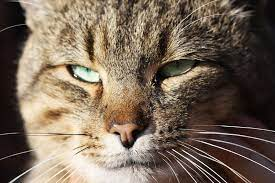
\includegraphics[width=0.5\textwidth]{téléchargement.jpeg}
    \caption{Qu'il est mignon}
    \label{fig:test}
\end{figure}
\lipsum[1][1-5]
\begin{table}[h]
    \centering
    \caption{Qu'il est mignon}
    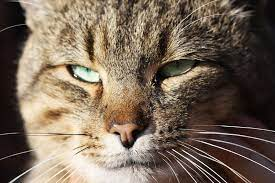
\includegraphics[width=0.5\textwidth]{téléchargement.jpeg}
   
    \label{fig:test}
\end{table}
\lipsum[1][1-5]
}

\begin{document}
\pagestyle{debut}
\loadgeometry{normal}
\justify
\sloppy
\pagestyle{main}

\chapter{final}
\section{Normal = 1}
\setstretch{1.2}
\setlength{\parskip}{4pt plus 2pt minus 2pt } 
\setlist{itemsep = 1pt plus 1pt minus 1pt, parsep = 1pt plus 1pt minus 1pt}
\setlength{\abovedisplayskip}{10pt plus 2pt minus 5pt}
\setlength{\abovedisplayshortskip}{10pt plus 2pt minus 5pt}
\setlength{\belowdisplayshortskip}{10pt plus 2pt minus 5pt}
\setlength{\belowdisplayskip}{10pt plus 2pt minus 5pt}
\setlength{\intextsep}{7pt plus 5pt minus 3pt}
\setlength{\textfloatsep}{5pt plus 7pt minus 1pt}
\setlength{\abovecaptionskip}{8pt plus 2pt minus 5pt}
\setlength{\belowcaptionskip}{8pt plus 2pt minus 5pt}
\lipsum[1-2]
\enumtest

\eqtest
\newpage
\figtest
\newpage
\section{petit = 0.5}
\setstretch{1}
\setlength{\parskip}{0pt plus 2pt } 
\setlist{itemsep = 1pt plus 1pt minus 1pt, parsep = 2pt plus 1pt minus 1pt}
\setlength{\abovedisplayskip}{2pt plus 2pt }
\setlength{\abovedisplayshortskip}{2pt plus 2pt }
\setlength{\belowdisplayshortskip}{2pt plus 2pt }
\setlength{\belowdisplayskip}{2pt plus 2pt }
\setlength{\intextsep}{2pt plus 5pt minus 3pt}
\setlength{\textfloatsep}{2pt plus 7pt minus 1pt}
\setlength{\abovecaptionskip}{6pt plus 2pt minus 5pt}
\setlength{\belowcaptionskip}{6pt plus 2pt minus 5pt}
\lipsum[1-2]
\enumtest

\eqtest
\newpage
\figtest

\newpage
\section{grand = 2}
\setstretch{1.5}
\setlength{\parskip}{10pt plus 3pt minus 3pt } 
\setlist{itemsep = 0pt plus 1pt minus 1pt, parsep = 0pt plus 1pt minus 1pt}
\setlength{\abovedisplayskip}{20pt plus 2pt minus 5pt}
\setlength{\abovedisplayshortskip}{20pt plus 2pt minus 10pt}
\setlength{\belowdisplayshortskip}{20pt plus 2pt minus 10pt}
\setlength{\belowdisplayskip}{15pt plus 2pt minus 5pt}
\setlength{\intextsep}{15pt plus 5pt minus 3pt}
\setlength{\textfloatsep}{10pt plus 7pt minus 1pt}
\setlength{\abovecaptionskip}{15pt plus 2pt minus 7pt}
\setlength{\belowcaptionskip}{15pt plus 2pt minus 7pt}
\lipsum[1-2]
\enumtest

\eqtest
\newpage
\figtest

\chapter{tests}
\section{test spacing}
\singlespacing
\lipsum[1-2]
\onehalfspacing
\lipsum[1-2]
\doublespacing
\lipsum[1-2]

\section{parskip}
\sbsec{parskip 1 }
\singlespacing
\setlength{\parskip}{0pt plus 1pt } 
\selectfont
\the\parskip \\
\lipsum[1-4]
\newpage
\sbsec{parskip 2 }
\setlength{\parskip}{4pt plus 2pt minus 2pt } 
\selectfont
\the\parskip \\
\lipsum[1-4]
\newpage
\sbsec{parskip 3 }
\setlength{\parskip}{8pt plus 3pt minus3pt } 
\selectfont
\the\parskip \\
\lipsum[1-2]


\section{enumeration}
\setlength{\parskip}{0pt plus 1pt }
\selectfont
\the\partopsep \\
\the\parskip \\
\the\topsep \\

\newpage
\sbsec{Enum 1 }
\singlespacing
\setlist{itemsep = 0mm, parsep = 0mm}
% \def\setItemsep{0mm}
% \def\setParsep{0mm}
%\selectfont

\enumtest
\newpage
\sbsec{Enum 2 }
\setlist{itemsep = 0.75mm, parsep = 1mm}
% \def\setItemsep{0.75mm} 
% \def\setParsep{1mm}
%\selectfont
\enumtest
\newpage
\sbsec{Enum 3 }
\setlist{itemsep = 1mm, parsep = 1.5mm}
% \def\setItemsep{5mm} 
% \def\setParsep{5mm} 
%\selectfont

\enumtest
\newpage
\sbsec{Enum 4 }
\setlist{nosep}
% \def\setItemsep{5mm} 
% \def\setParsep{5mm} 
%\selectfont

\enumtest
\sbsec{Enum 5 }
\setlist{noitemsep} 
% \def\setItemsep{5mm} 
% \def\setParsep{5mm} 
%\selectfont


\newpage
\sbsec{Enum 4 }
\setlength{\parskip}{8pt plus 3pt minus3pt } 
\selectfont
\setlist{nosep}
% \def\setItemsep{5mm} 
% \def\setParsep{5mm} 
%\selectfont

\enumtest
\sbsec{Enum 5 }
\setlist{noitemsep} 
% \def\setItemsep{5mm} 
% \def\setParsep{5mm} 
%\selectfont

\enumtest
\section{equation}
\newpage
\sbsec{eq1}
\the\parskip
\setlength{\abovedisplayskip}{0pt}
\setlength{\abovedisplayshortskip}{0pt }
\setlength{\belowdisplayshortskip}{0pt }
\setlength{\belowdisplayskip}{0pt}
\eqtestsp
\newpage
\sbsec{eq1}
\setlength{\parskip}{0pt plus 1pt } 
\selectfont
\the\parskip
\setlength{\abovedisplayskip}{1pt}
\setlength{\abovedisplayshortskip}{1pt }
\setlength{\belowdisplayshortskip}{1pt }
\setlength{\belowdisplayskip}{1pt}
\the\belowdisplayskip
\the\abovedisplayskip

\eqtest


le \\\\ à la fin de l'équation crée des espaces supplémentaires
\newpage

\sbsec{eq2}
\the\parskip
\setlength{\abovedisplayskip}{10pt}
\setlength{\abovedisplayshortskip}{10pt }
\setlength{\belowdisplayshortskip}{10pt }
\setlength{\belowdisplayskip}{10pt}
\eqtest
\newpage
\sbsec{eq3}
\the\parskip
\setlength{\abovedisplayskip}{15pt}
\setlength{\abovedisplayshortskip}{15pt }
\setlength{\belowdisplayshortskip}{15pt }
\setlength{\belowdisplayskip}{15pt}
\eqtest
\newpage 
\setlength{\parskip}{8pt plus 3pt minus3pt } 
\selectfont
\sbsec{eq2 : \the\parskip}
\the\parskip
\setlength{\abovedisplayskip}{10pt}
\setlength{\abovedisplayshortskip}{10pt }
\setlength{\belowdisplayshortskip}{10pt }
\setlength{\belowdisplayskip}{10pt}
\eqtest
\newpage
\sbsec{eq3 : \the\parskip}
\the\parskip
\setlength{\abovedisplayskip}{15pt}
\setlength{\abovedisplayshortskip}{15pt }
\setlength{\belowdisplayshortskip}{15pt }
\setlength{\belowdisplayskip}{15pt}
\eqtest

\section{figure}
\newpage
\setlength{\parskip}{0pt plus 1pt } 
\selectfont

\setlength{\intextsep}{0pt}
\setlength{\textfloatsep}{0pt}  
\setlength{\abovecaptionskip}{0pt}
\setlength{\belowcaptionskip}{0pt}
\the\abovecaptionskip \the\belowcaptionskip
\figtest
\newpage

\setlength{\intextsep}{10pt}
\setlength{\textfloatsep}{10pt}
\setlength{\abovecaptionskip}{0pt}
\setlength{\belowcaptionskip}{0pt}
\the\abovecaptionskip \the\belowcaptionskip
\figtest
\newpage

\setlength{\intextsep}{10pt}
\setlength{\textfloatsep}{10pt}
\setlength{\abovecaptionskip}{10pt}
\setlength{\belowcaptionskip}{0pt}
\the\abovecaptionskip \the\belowcaptionskip
\figtest
\newpage
\setlength{\intextsep}{10pt}
\setlength{\textfloatsep}{10pt}
\setlength{\abovecaptionskip}{10pt}
\setlength{\belowcaptionskip}{10pt}
\the\abovecaptionskip \the\belowcaptionskip
\figtest
\end{document}
